\section{Anexo: catálogo y fichas de las simulaciones}\label{sec:anexo}

La tabla~\ref{tab:catalogo} lista las 65 simulaciones de cribado, ciudad completa y cuadratura; las 19 microsimulaciones del campus se describen en el texto. A continuación, cada simulación clave tiene una ficha con su lámina: el barro simulado (espesor máximo) sobre la zona afectada oficial de IDE Chile y los ejes viales afectados, qué prueba, qué muestra, qué limitaciones presenta y qué hipótesis levanta. Los ensayos v25 a v29 y las microsimulaciones del campus se resumen en las secciones~\ref{sec:res-ronda} y~\ref{sec:res-posterior}; v22 a v24 se detuvieron antes de terminar (registro de experimentos).

{\scriptsize\setlength{\tabcolsep}{2.5pt}
\begin{longtable}{lll>{\raggedright\arraybackslash}p{3.3cm}rlrrrrrrr}
\caption{Catálogo de las 65 simulaciones de cribado, ciudad completa y cuadratura (las 19 microsimulaciones del campus se describen en la sección~\ref{sec:res-posterior}), ordenadas por índice exploratorio de compatibilidad (IEC). Las capacidades del colector y los escenarios sin incendio son supuestos de cálculo; no describen obras reales ni establecen contrafactuales del evento. Columnas como en la tabla~\ref{tab:v4}; las corridas con paso normal cuyo componente «sitios» depende del punto de control del campus no se usan para seleccionar con su IEC bruto: sin ese punto obtienen 71--76, salvo verificación con paso fino (z26: 76; z29: 78) (enmienda 1 del protocolo); v31 se descartó (inyección del cauce principal fuera del fondo de la quebrada); las corridas posteriores a la prueba reservada son de ajuste; Fecha: día y mes en que terminó la simulación (2026). Terreno: ciudad (42.018 edificios), anterior (1.103 edificios), ant.+cauce (anterior con el cauce del parque lineal tallado) o SPOT 2014.}\label{tab:catalogo}\\\toprule
Terr. & Fecha & Corrida & Escenario & $V$ (mil m$^3$) & Barro & Calles & Sitios & dPH (m) & Perím. & QH & UCC (m) & IEC\\\midrule\endfirsthead
\toprule Terr. & Fecha & Corrida & Escenario & $V$ (mil m$^3$) & Barro & Calles & Sitios & dPH (m) & Perím. & QH & UCC (m) & IEC\\\midrule\endhead
ciudad & 11-10 & v26 & cauce + brazos sur; casas porosas en la zona oficial + lluvia neta & 300 & G2b & 0{,}77 & 1{,}00 & 1 & 0{,}54 & 0{,}56 & 0{,}30 & 83\\
ciudad & 12-10 & v30 & cauce + brazos sur; casas porosas, Kp 1000 y n 0,1 (sensibilidad de v26) & 300 & G2b & 0{,}76 & 1{,}00 & 1 & 0{,}53 & 0{,}54 & 0{,}31 & 82\\
ciudad & 12-10 & v32 & cauce + brazos sur; hipótesis integrada: casas porosas, faldeo agua turbia, camino, La Plaza Sur y entradas a la universidad & 300 & G2b & 0{,}77 & 1{,}00 & 1 & 0{,}51 & 0{,}56 & 0{,}30 & 82\\
ciudad & 12-10 & z32 & cauce + brazos sur; hipótesis integrada, paso fino & 300 & G2b & 0{,}77 & 1{,}00 & 5 & 0{,}51 & 0{,}56 & 0{,}30 & 82\\
ciudad & 13-10 & f35 & cauce + brazos sur; como p34, sin incendio: 187 mil m³ y Qp 172 m$^3$/s; con artefacto de +3,1 \%, repetida como f35b/f38b & 187 & G2b & 0{,}73 & 1{,}00 & 5 & 0{,}53 & 0{,}56 & 0{,}23 & 82\\
ciudad & 13-10 & m36 & cauce + brazos sur; como p34, con malla fina (8 m²) en el campus y La Plaza Sur & 300 & G2b & 0{,}78 & 1{,}00 & 6 & 0{,}48 & 0{,}52 & 0{,}32 & 82\\
ciudad & 13-10 & f35b & cauce + brazos sur; repetición corregida de f35, sin incendio & 187 & G2b & 0{,}73 & 1{,}00 & 5 & 0{,}55 & 0{,}56 & 0{,}23 & 82\\
ciudad & 13-10 & d39 & cauce + brazos sur; como p34, porosas solo las casas de 250 m² o menos & 300 & G2b & 0{,}77 & 1{,}00 & 5 & 0{,}47 & 0{,}55 & 0{,}31 & 81\\
ciudad & 13-10 & p34 & cauce + brazos sur; hipótesis integrada con la lluvia medida en Río Molina cada 30 min (31,8 mm); con artefacto de +2,1 \% de masa, repetida sin él como p34b & 300 & G2b & 0{,}77 & 1{,}00 & 1 & 0{,}48 & 0{,}56 & 0{,}30 & 81\\
ciudad & 13-10 & p34b & cauce + brazos sur; repetición corregida de p34 (paso máximo 0,5 s, residuo 0,00 \%) & 300 & G2b & 0{,}77 & 1{,}00 & 1 & 0{,}48 & 0{,}56 & 0{,}30 & 81\\
ciudad & 13-10 & f38 & cauce + brazos sur; como f35, barro más fluido (Cv 0,25); con artefacto de +3,1 \%, repetida como f35b/f38b & 187 & G2b & 0{,}70 & 1{,}00 & 5 & 0{,}49 & 0{,}54 & 0{,}19 & 80\\
ciudad & 13-10 & f38b & cauce + brazos sur; repetición corregida de f38, sin incendio y barro más fluido & 187 & G2b & 0{,}70 & 1{,}00 & 5 & 0{,}50 & 0{,}54 & 0{,}19 & 80\\
ciudad & 11-10 & v27 & cauce + brazos sur; más rugosidad en jardines y árboles + lluvia & 300 & G2b & 0{,}78 & 1{,}00 & 8 & 0{,}39 & 0{,}68 & 1{,}13 & 79\\
ciudad & 12-10 & v33 & cauce + brazos sur; hipótesis integrada con lluvia medida: 8 mm/h durante 4 h & 300 & G2b & 0{,}76 & 1{,}00 & 1 & 0{,}41 & 0{,}56 & 0{,}30 & 79\\
ciudad & 13-10 & arc & cauce + brazos sur; como p34, cauce principal tallado por la línea de árboles e inyectado aguas arriba (control del obstáculo hipotético) & 300 & G2b & 0{,}75 & 1{,}00 & 5 & 0{,}40 & 0{,}56 & 0{,}24 & 79\\
ciudad & 11-10 & v20 & cauce + brazos sur; lluvia 35 mm/h + brazo sur oficial (terreno v6), paso normal & 300 & G2b & 0{,}77 & 1{,}00 & 15 & 0{,}33 & 0{,}68 & 1{,}12 & 78\\
ciudad & 11-10 & v25 & cauce + brazos sur; barro algo más denso (Cv 0,43) + lluvia & 300 & G2b & 0{,}77 & 1{,}00 & 15 & 0{,}35 & 0{,}68 & 1{,}11 & 78\\
ciudad & 11-10 & v29 & cauce + brazos sur; faldeo líquido (Cv 0,27) + rama principal Cv 0,43 + lluvia neta & 300 & G2b & 0{,}77 & 1{,}00 & 15 & 0{,}35 & 0{,}68 & 1{,}11 & 78\\
ciudad & 11-10 & v28 & cauce + brazos sur; lluvia 35 mm/h solo fuera de las cuencas aportantes (sin doble conteo) & 300 & G2b & 0{,}77 & 1{,}00 & 15 & 0{,}34 & 0{,}68 & 1{,}13 & 78\\
ciudad & 11-10 & q3 & cauce + brazos sur; cuadratura de Cv: nodo Cv 0,365 & 300 & G2b & 0{,}77 & 1{,}00 & 15 & 0{,}34 & 0{,}68 & 1{,}13 & 78\\
ciudad & 11-10 & q4 & cauce + brazos sur; cuadratura de Cv: nodo Cv 0,429 & 300 & G2b & 0{,}77 & 1{,}00 & 15 & 0{,}36 & 0{,}68 & 1{,}12 & 78\\
ciudad & 12-10 & z29 & cauce + brazos sur; faldeo Cv 0,27, paso fino & 300 & G2b & 0{,}77 & 1{,}00 & 15 & 0{,}35 & 0{,}68 & 1{,}11 & 78\\
ciudad & 12-10 & v31 & cauce + brazos sur; hipótesis integrada: casas porosas, camino, La Plaza Sur, entradas a la universidad, árboles, H1 aguas arriba, faldeo Cv 0,10 & 300 & G2b & 0{,}72 & 1{,}00 & 191 & 0{,}40 & 0{,}51 & 0{,}19 & 78\\
ciudad & 13-10 & art & cauce + brazos sur; como arc, con obstáculo hipotético de troncos de altura supuesta de 3 m al final de la línea de árboles & 300 & G2b & 0{,}73 & 1{,}00 & 5 & 0{,}39 & 0{,}54 & 0{,}22 & 78\\
ciudad & 11-10 & q2 & cauce + brazos sur; cuadratura de Cv: nodo Cv 0,297 & 300 & G2b & 0{,}77 & 1{,}00 & 15 & 0{,}32 & 0{,}68 & 1{,}14 & 77\\
ciudad & 11-10 & q1 & cauce + brazos sur; cuadratura de Cv: nodo Cv 0,239 & 300 & G2b & 0{,}76 & 1{,}00 & 15 & 0{,}32 & 0{,}68 & 1{,}14 & 77\\
ciudad & 12-10 & z26 & cauce + brazos sur; casas porosas, paso fino & 300 & G2b & 0{,}76 & 0{,}75 & 5 & 0{,}54 & 0{,}56 & 0{,}30 & 76\\
ciudad & 11-10 & q5 & cauce + brazos sur; cuadratura de Cv: nodo Cv 0,478 & 300 & G2b & 0{,}78 & 0{,}75 & 34 & 0{,}38 & 0{,}68 & 1{,}11 & 73\\
ciudad & 10-10 & v02 & cauce + brazos sur; lluvia 35 mm/h en ladera & 300 & G2b & 0{,}77 & 0{,}75 & 15 & 0{,}34 & 0{,}68 & 1{,}13 & 72\\
ciudad & 10-10 & z02 & cauce + brazos sur; lluvia 35 mm/h, paso 4× más fino & 300 & G2b & 0{,}77 & 0{,}75 & 15 & 0{,}34 & 0{,}68 & 1{,}13 & 72\\
anterior & 09-10 & f03 & abanico + embocadura + brazos sur; lluvia 35 mm/h en ladera & 150 & G2b & 0{,}73 & 0{,}75 & 225 & 0{,}39 & 0{,}66 & 0{,}26 & 71\\
ciudad & 10-10 & v14 & cauce + brazos sur; lluvia 35 mm/h + quebrada Álvaro del Portillo & 300 & G2b & 0{,}77 & 0{,}75 & 15 & 0{,}34 & 0{,}68 & 1{,}15 & 71\\
ciudad & 11-10 & v19 & cauce + brazos sur; lluvia 35 mm/h + brazo sur oficial hasta Álvaro del Portillo (terreno v6) & 300 & G2b & 0{,}77 & 0{,}75 & 15 & 0{,}34 & 0{,}68 & 1{,}11 & 71\\
ciudad & 10-10 & v09 & cauce principal & 300 & A2 & 0{,}77 & 0{,}50 & 151 & 0{,}52 & 0{,}68 & 1{,}14 & 70\\
ciudad & 10-10 & v03 & cauce principal; colector con capacidad supuesta de 30 m$^3$/s & 300 & G2b & 0{,}77 & 0{,}50 & 96 & 0{,}50 & 0{,}64 & 1{,}16 & 69\\
ciudad & 10-10 & v05 & cauce principal; colector con capacidad supuesta de 100 m$^3$/s & 300 & G2b & 0{,}74 & 0{,}50 & 96 & 0{,}53 & 0{,}44 & 1{,}16 & 69\\
ciudad & 10-10 & v06 & cauce principal; colector con capacidad supuesta de 60 m$^3$/s & 300 & G2b & 0{,}74 & 0{,}50 & 96 & 0{,}53 & 0{,}44 & 1{,}16 & 69\\
ciudad & 10-10 & v17 & cauce principal; colector con capacidad supuesta de 30 m$^3$/s, captura 25 m, Quebrada Honda tallada & 300 & G2b & 0{,}76 & 0{,}50 & 96 & 0{,}50 & 0{,}62 & 1{,}18 & 69\\
ant.+cauce & 09-10 & f01 & cauce principal & 150 & G2b & 0{,}71 & 0{,}50 & 338 & 0{,}63 & 0{,}55 & 0{,}31 & 68\\
ant.+cauce & 09-10 & e04 & cauce principal & 300 & G2b & 0{,}75 & 0{,}50 & 2 & 0{,}46 & 0{,}56 & 0{,}32 & 68\\
ciudad & 10-10 & v01 & cauce principal & 300 & G2b & 0{,}77 & 0{,}50 & 96 & 0{,}46 & 0{,}68 & 1{,}16 & 68\\
ciudad & 10-10 & z01 & cauce principal; control numérico (paso 4× más fino) & 300 & G2b & 0{,}77 & 0{,}50 & 96 & 0{,}46 & 0{,}68 & 1{,}16 & 68\\
ciudad & 10-10 & v10 & cauce principal; colector con capacidad supuesta de 100 m$^3$/s, captura 25 m & 300 & G2b & 0{,}69 & 0{,}50 & 96 & 0{,}52 & 0{,}00 & 1{,}16 & 68\\
ciudad & 10-10 & v11 & cauce principal; colector con capacidad supuesta de 200 m$^3$/s, captura 40 m & 300 & G2b & 0{,}69 & 0{,}50 & 96 & 0{,}52 & 0{,}00 & 1{,}16 & 68\\
ciudad & 10-10 & v15 & cauce principal; Quebrada Honda tallada aguas abajo (terreno v5) & 300 & G2b & 0{,}77 & 0{,}50 & 96 & 0{,}45 & 0{,}68 & 1{,}18 & 68\\
ciudad & 10-10 & v18 & cauce principal; colector con capacidad supuesta de 100 m$^3$/s, captura 25 m, Quebrada Honda tallada & 300 & G2b & 0{,}69 & 0{,}50 & 96 & 0{,}52 & 0{,}00 & 1{,}18 & 68\\
ciudad & 11-10 & v21 & cauce + brazos sur; brazo sur oficial (terreno v6), sin lluvia & 300 & G2b & 0{,}77 & 0{,}50 & 131 & 0{,}45 & 0{,}68 & 1{,}11 & 68\\
ant.+cauce & 09-10 & k03 & cauce principal; colector con capacidad supuesta de 10 m$^3$/s & 150 & G2b & 0{,}70 & 0{,}50 & 338 & 0{,}64 & 0{,}43 & 0{,}31 & 67\\
ciudad & 10-10 & v07 & cauce principal & 150 & G2b & 0{,}72 & 0{,}50 & 348 & 0{,}62 & 0{,}68 & 1{,}09 & 67\\
ciudad & 10-10 & v08 & cauce principal & 300 & G1 & 0{,}74 & 0{,}50 & 396 & 0{,}63 & 0{,}69 & 1{,}16 & 67\\
ant.+cauce & 09-10 & k01 & cauce principal; colector con capacidad supuesta de 30 m$^3$/s & 150 & G2b & 0{,}65 & 0{,}50 & 338 & 0{,}63 & 0{,}01 & 0{,}31 & 66\\
ant.+cauce & 09-10 & k02 & cauce principal; colector con capacidad supuesta de 100 m$^3$/s & 150 & G2b & 0{,}65 & 0{,}50 & 338 & 0{,}63 & 0{,}01 & 0{,}31 & 66\\
anterior & 09-10 & d02 & cauce + brazos sur & 300 & G2b & 0{,}68 & 0{,}50 & 4 & 0{,}41 & 0{,}00 & 0{,}42 & 65\\
anterior & 09-10 & d04 & cauce principal & 150 & G2b & 0{,}63 & 0{,}50 & 366 & 0{,}55 & 0{,}00 & 0{,}42 & 63\\
anterior & 09-10 & d01 & cauce + brazos sur & 150 & G2b & 0{,}60 & 0{,}50 & 516 & 0{,}55 & 0{,}00 & 0{,}39 & 58\\
anterior & 09-10 & g01 & cauce + brazos sur & 150 & G2b & 0{,}58 & 0{,}50 & 592 & 0{,}51 & 0{,}00 & 0{,}38 & 55\\
anterior & 09-10 & g03 & abanico + embocadura + brazos sur & 150 & G2b & 0{,}60 & 0{,}50 & 816 & 0{,}53 & 0{,}54 & 0{,}35 & 50\\
anterior & 09-10 & f02 & abanico + embocadura + brazos sur; lluvia 20 mm/h en ladera & 150 & G2b & 0{,}56 & 0{,}75 & 1005 & 0{,}46 & 0{,}66 & 0{,}26 & 49\\
anterior & 09-10 & g02 & abanico + embocadura + brazos sur & 150 & G2b & 0{,}61 & 0{,}50 & 947 & 0{,}51 & 0{,}57 & 0{,}33 & 47\\
anterior & 09-10 & e06 & cauce principal & 150 & G1 & 0{,}47 & 0{,}50 & 1686 & 0{,}80 & 0{,}45 & 0{,}59 & 44\\
anterior & 09-10 & d03 & cauce + brazos sur; caudal pico 100 m$^3$/s & 80 & G2b & 0{,}50 & 0{,}50 & 1160 & 0{,}68 & 0{,}00 & 0{,}22 & 43\\
anterior & 09-10 & e01 & abanico + embocadura + brazos sur & 150 & G2b & 0{,}56 & 0{,}50 & 1007 & 0{,}46 & 0{,}66 & 0{,}26 & 43\\
anterior & 09-10 & e02 & abanico + embocadura + brazos sur & 150 & G2b & 0{,}52 & 0{,}50 & 982 & 0{,}43 & 0{,}67 & 0{,}23 & 42\\
SPOT 2014 & 09-10 & s01 & cauce principal & 150 & G2b & 0{,}50 & 0{,}50 & 1188 & 0{,}60 & 0{,}77 & 0{,}37 & 40\\
anterior & 09-10 & e03 & solo embocadura & 150 & G2b & 0{,}08 & 0{,}00 & 856 & 0{,}20 & 0{,}69 & 0{,}00 & 16\\
\bottomrule\end{longtable}}


\subsection*{Ensayos posteriores a la prueba reservada (ajuste)}

\paragraph{v32 · Hipótesis integrada: casas porosas, agua turbia en el faldeo y rasgos del campus.} \textbf{Qué prueba:} Reúne lo aprendido después de la prueba reservada: casas de la zona oficial que dejan entrar el barro, agua turbia (Cv 0,10) en el faldeo del campus y La Plaza Sur, barro de Cv 0,40 en la rama principal, y los rasgos que el relieve de 30 m no resuelve (camino del cerro, calzada baja de La Plaza Sur, entradas a la universidad y al estacionamiento), con lluvia sobre todo el faldeo fuera de las cuencas aportantes. \textbf{Qué muestra:} Calculado: cumple los cuatro criterios originales (IEC 82/100; la repetición con paso fino, z32, da el mismo valor); el barro urbano dentro de la zona oficial llega a 51 \%; el campus marca 0,61 m; La Plaza Sur se moja en el 46 \% de su largo; en el modelo, el agua entra por el claro al patio (0,07 m) y al estacionamiento. \textbf{Limitaciones del modelo:} Junto a la urgencia de la UC Christus calcula 0,30 m (Cadena 3 informó cerca de 1 m en urgencias). En el campus, con la malla de ciudad, llega menos agua que en las simulaciones de detalle; con malla fina en el campus (m36) el patio llega a 0,17 m, lo que atribuye la diferencia a la resolución. Está condicionada a una lluvia de 35 mm/h durante una hora, mayor que la medida: con la lluvia medida obtiene 79/100 (repartida de forma pareja) u 81/100 (con su forma de pulso). \textbf{Qué levanta:} En el modelo se asignan propiedades distintas al flujo de la rama principal y al del campus; la retención supuesta en los lotes modifica la distribución calculada dentro de la zona oficial. El ajuste no identifica los procesos ocurridos durante el evento. \textbf{Estado:} IEC 82/100 verificado con paso fino (z32). Ajuste posterior a la prueba reservada.

\begin{figure}[H]\centering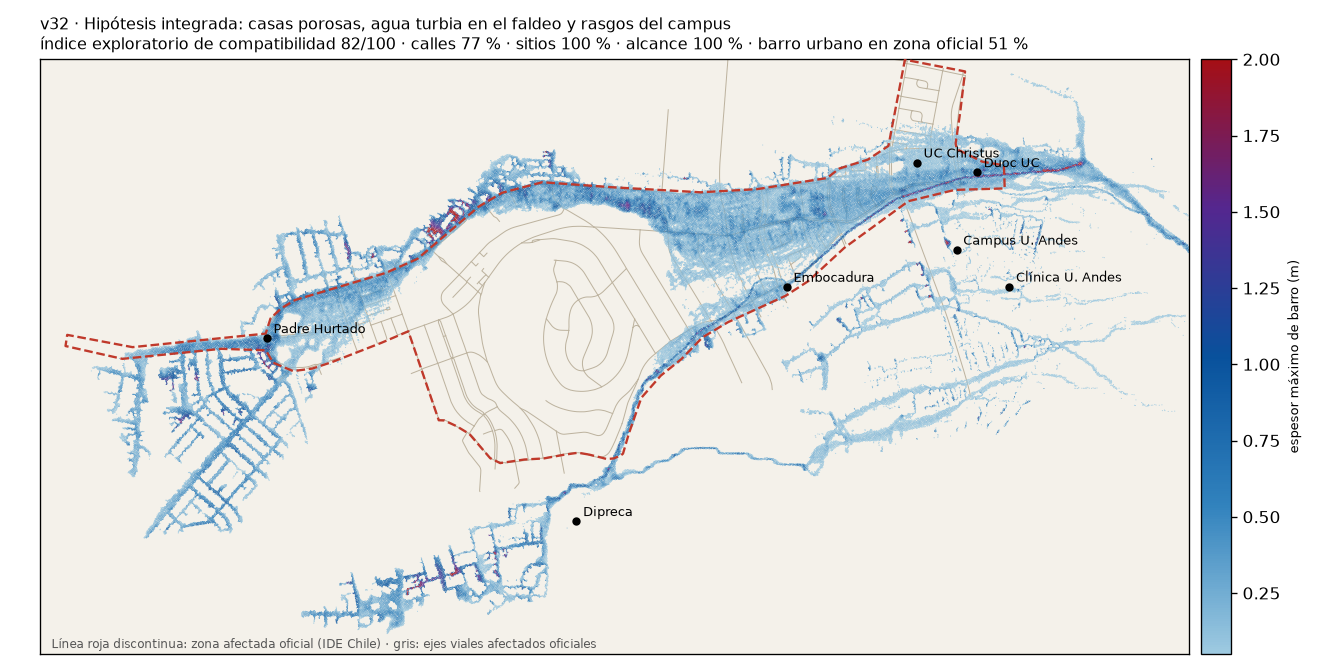
\includegraphics[width=\textwidth]{anexo/v32}\caption{Ficha v32: Hipótesis integrada: casas porosas, agua turbia en el faldeo y rasgos del campus.}\end{figure}

\paragraph{z26 · Casas porosas (paso fino).} \textbf{Qué prueba:} Que los edificios de la zona oficial dejen entrar el barro (piso a la cota del terreno más 0,3 m y alta resistencia), en vez de ser bloques macizos. \textbf{Qué muestra:} Calculado: el barro urbano dentro de la zona oficial sube de 34 \% a 54 \%; moja el 36 \% del área oficial y el 40 \% de sus predios afectados; cumple los cuatro criterios originales. Con la mitad de la resistencia (v30) casi no cambia. \textbf{Limitaciones del modelo:} El espesor calculado junto a la urgencia de la UC Christus baja a 0,30 m. El punto del campus no se moja con paso fino. \textbf{Qué levanta:} En el modelo, la retención supuesta de barro en los lotes modifica la distribución calculada dentro de la zona oficial; su representación sigue siendo un supuesto. \textbf{Estado:} IEC verificado con paso fino: 76/100 (ajuste posterior).

\begin{figure}[H]\centering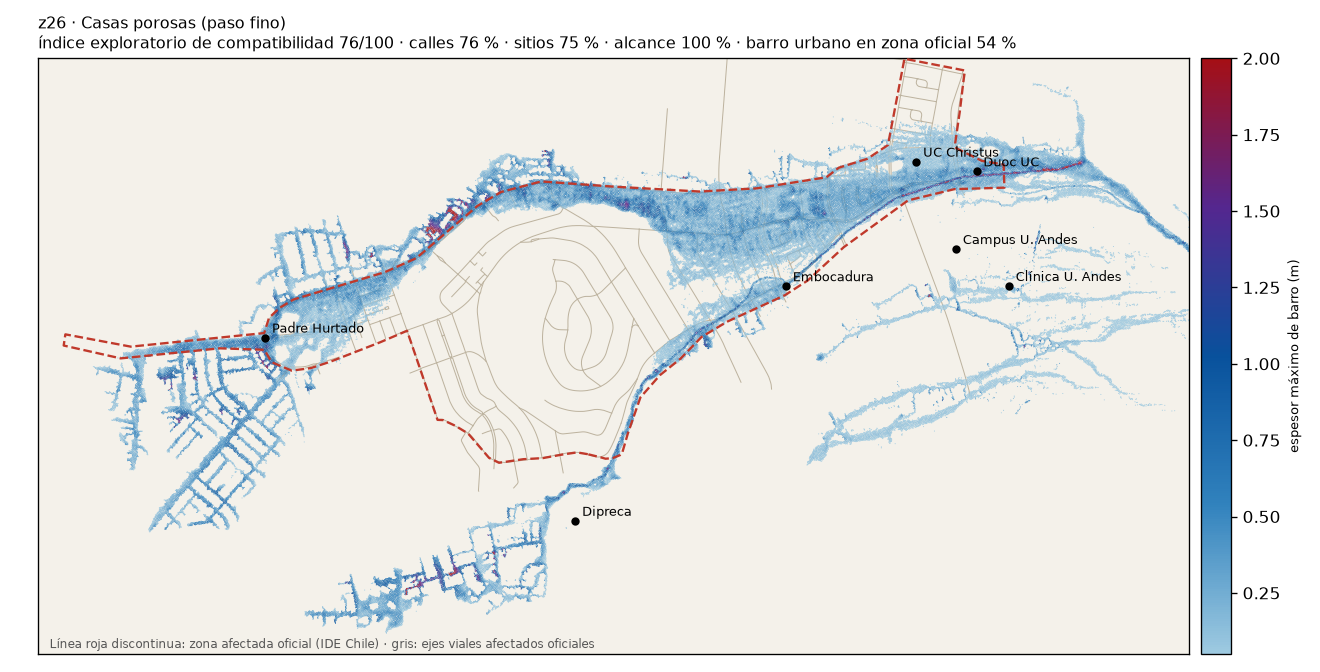
\includegraphics[width=\textwidth]{anexo/z26}\caption{Ficha z26: Casas porosas (paso fino).}\end{figure}

\paragraph{z29 · Faldeo más líquido (paso fino).} \textbf{Qué prueba:} Dos barros según la zona: Cv 0,27 en el faldeo del campus y Cv 0,43 en la rama principal, con la lluvia solo fuera de las cuencas aportantes. \textbf{Qué muestra:} Calculado: el punto de control del campus se mantiene mojado con paso fino (0,09 m), a diferencia de la hipótesis con un solo barro (0,01 m). \textbf{Limitaciones del modelo:} No reduce el barro fuera de la zona oficial: la fracción dentro de ella queda en 0,35. \textbf{Qué levanta:} En estos ensayos, un fluido supuesto más líquido en el faldeo, compatible con el agua turbia interpretada en el video de Meganoticias, produce flujo en el campus también con paso fino. \textbf{Estado:} IEC verificado con paso fino: 78/100 (ajuste posterior).

\begin{figure}[H]\centering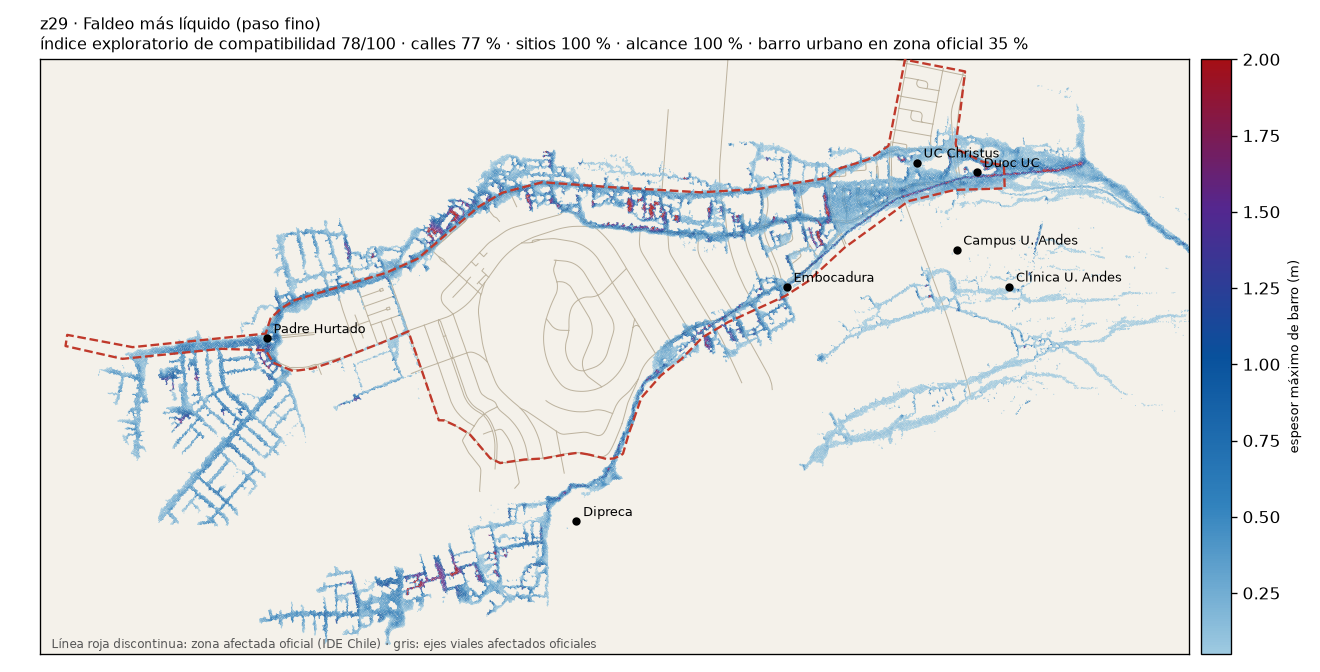
\includegraphics[width=\textwidth]{anexo/z29}\caption{Ficha z29: Faldeo más líquido (paso fino).}\end{figure}

\subsection*{Hipótesis seleccionada para la prueba reservada}

\paragraph{z02 · Cauce + brazos sur + lluvia en ladera, ciudad completa (paso fino).} \textbf{Qué prueba:} La hipótesis seleccionada antes de la prueba con observaciones reservadas: el barro sale por el cauce principal al abanico y por los brazos sur, y además se aplica una lluvia de 35 mm/h sobre la ladera quemada. Repite v02 con un paso de tiempo cuatro veces más fino para examinar la sensibilidad al paso de tiempo. \textbf{Qué muestra:} Calculado: el flujo simulado recorre los dos corredores que delimitan la zona oficial (El Alba–General Blanche y Quebrada Honda) y llega a menos de 200 m de Padre Hurtado; en el entorno de la Clínica UC Christus calcula 1,13 m (Cadena 3 informó cerca de 1 m en urgencias) y produce flujo junto a la Clínica U. de los Andes. Los indicadores coinciden con los de v02; esta comprobación numérica no valida la reconstrucción del evento. \textbf{Limitaciones del modelo:} Solo un tercio del barro simulado en zona urbana cae dentro de la zona oficial: se extiende al poniente de Padre Hurtado, por Quebrada Honda hacia Dipreca y, por la lluvia aplicada, por calles de otros barrios. No alcanza el campus de la U. de los Andes. Parte de la lluvia aplicada (unos 9.400 m$^3$) se superpone con cuencas que ya entran por los hidrogramas; v28 lo corrige. \textbf{Qué levanta:} En z02, el aporte de lluvia sobre la ladera contribuye a reproducir el flujo junto a la clínica; el resultado no establece su participación durante el evento. Como posibles explicaciones de la extensión fuera de la zona oficial se consideran la representación de los edificios, la carga gruesa y la vegetación (v25–v27). \textbf{Estado:} Hipótesis seleccionada antes de la prueba con observaciones reservadas (prueba desfavorable): IEC 72/100. Los ensayos posteriores (casas porosas, faldeo líquido, hipótesis integrada) la superan, como ajuste.

\begin{figure}[H]\centering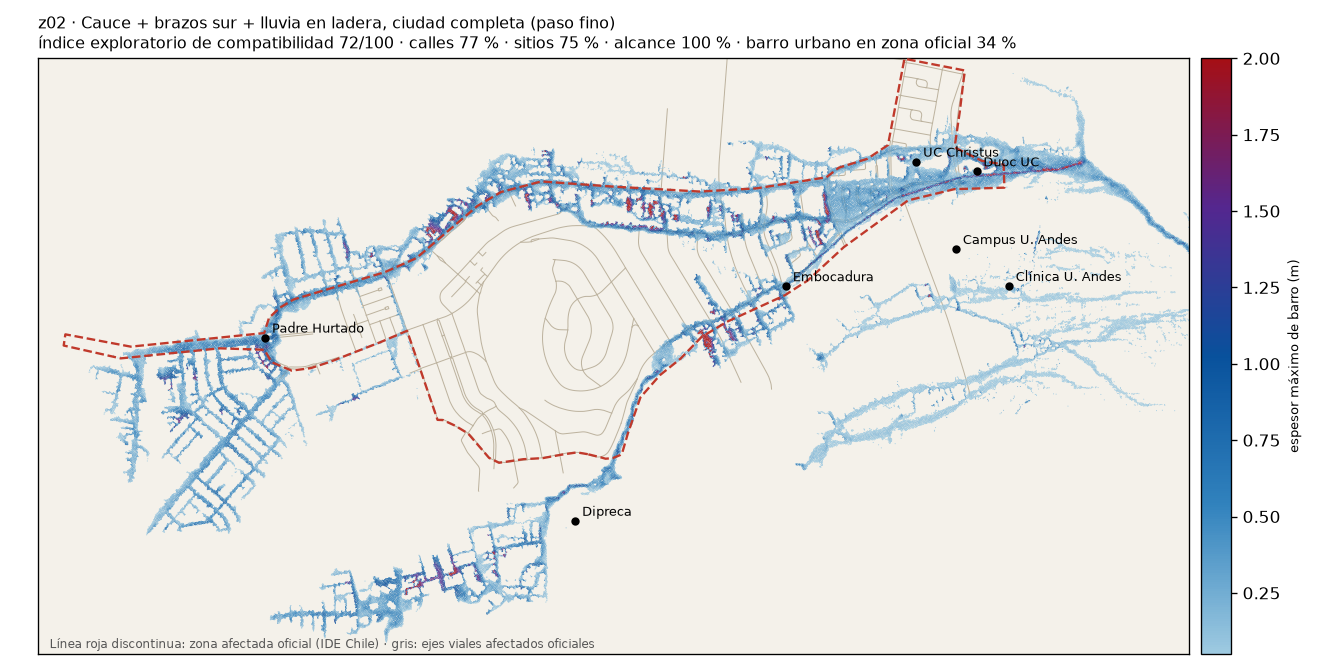
\includegraphics[width=\textwidth]{anexo/z02}\caption{Ficha z02: Cauce + brazos sur + lluvia en ladera, ciudad completa (paso fino).}\end{figure}

\subsection*{Ciudad completa}

\paragraph{v01 · Solo cauce principal, colector con capacidad nula supuesta (300 mil m$^3$).} \textbf{Qué prueba:} Todo el barro sale por el cauce principal al abanico, con los ductos de General Blanche y el colector de Bulnes Correa con capacidad nula supuesta (escenario hipotético). \textbf{Qué muestra:} Calculado: con los 42 mil edificios, el flujo se encauza por las calles; calcula 1,16 m en el entorno de la UC Christus (0,3 m con el terreno anterior), 1,9 m junto a Duoc UC, llega a 96 m de Padre Hurtado y moja Quebrada Honda. \textbf{Limitaciones del modelo:} No reproduce la afectación junto a la Clínica U. de los Andes, en La Plaza Sur ni en el campus. \textbf{Qué levanta:} Esta configuración no reproduce la afectación del sector sur. Los aportes desde ese sector constituyen una de las hipótesis consideradas para explicar la discrepancia. \textbf{Estado:} Referencia: IEC 68/100.

\begin{figure}[H]\centering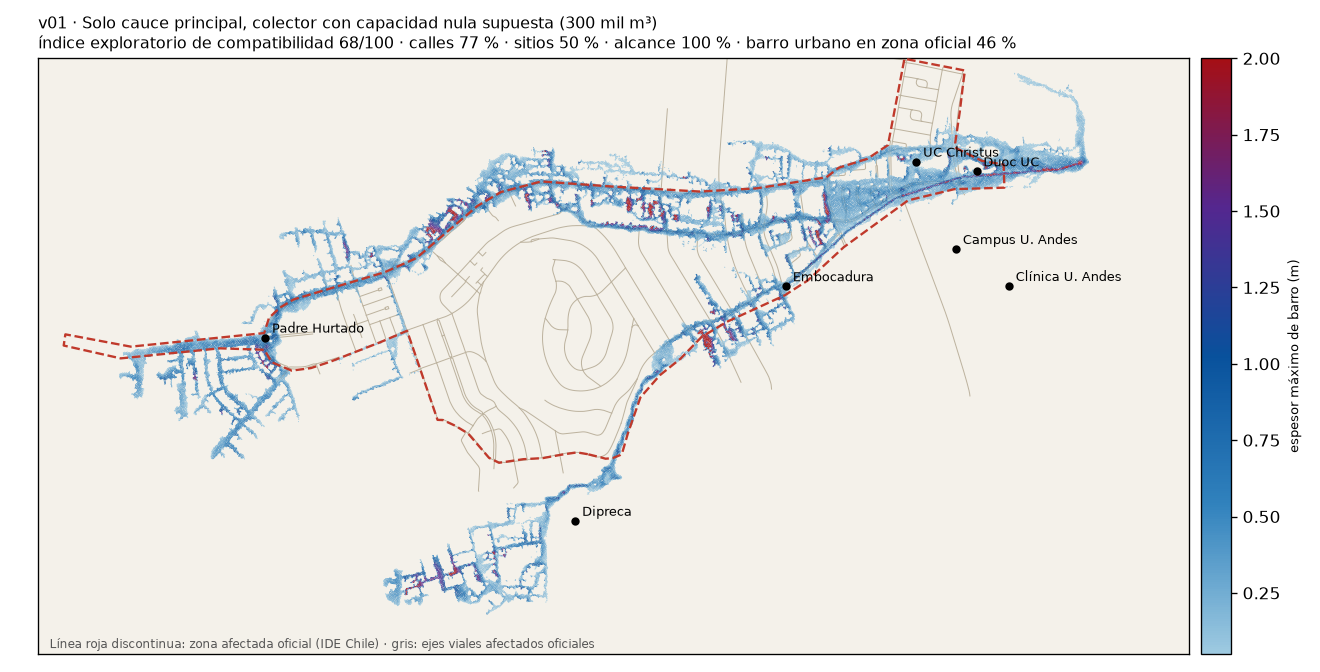
\includegraphics[width=\textwidth]{anexo/v01}\caption{Ficha v01: Solo cauce principal, colector con capacidad nula supuesta (300 mil m$^3$).}\end{figure}

\paragraph{v07 · Solo cauce principal con 150 mil m$^3$.} \textbf{Qué prueba:} Igual que v01, pero con la mitad del volumen: el valor central de la primera estimación por lluvia. \textbf{Qué muestra:} Calculado: el frente se detiene a 348 m de Padre Hurtado. \textbf{Limitaciones del modelo:} No cumple el criterio de alcance. \textbf{Qué levanta:} En los escenarios ensayados y bajo sus supuestos, unos 300 mil m$^3$ permiten reproducir el criterio de alcance; ese orden de magnitud es coherente con una estimación por lluvia que adopta la saturación del suelo informada por la autoridad. \textbf{Estado:} La configuración con el volumen bajo no cumple el criterio de alcance: IEC 67/100.

\begin{figure}[H]\centering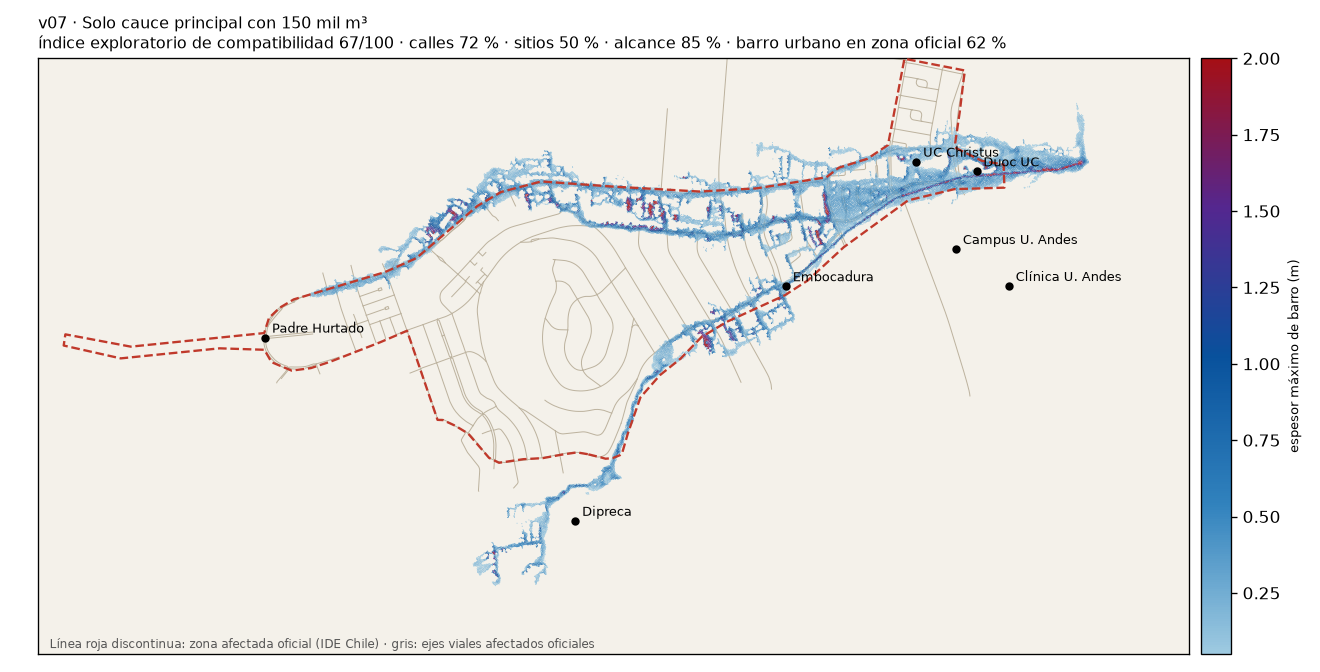
\includegraphics[width=\textwidth]{anexo/v07}\caption{Ficha v07: Solo cauce principal con 150 mil m$^3$.}\end{figure}

\subsection*{Campus U. Andes}

\paragraph{v21 · Brazo sur por el cauce oficial, sin lluvia en ladera.} \textbf{Qué prueba:} El brazo sur sigue el trazado de la red hidrográfica oficial hasta la parte alta de la Av. Álvaro del Portillo, donde termina el trazado oficial y el modelo deja salir el flujo a la avenida. Sin lluvia en la ladera, para aislar su efecto. \textbf{Qué muestra:} Calculado: el barro del brazo sur llega a la avenida (0,48 m donde termina el cauce) y baja por ella hacia La Plaza y General Blanche, de forma compatible con lo atribuido al vicerrector por Cooperativa y a Carabineros por La Tercera. \textbf{Limitaciones del modelo:} Sin la lluvia en la ladera no se reproduce la afectación junto a la Clínica U. de los Andes (0 m) y el flujo no alcanza la Biblioteca. \textbf{Qué levanta:} En las configuraciones comparadas, la lluvia sobre la ladera permite reproducir la afectación junto a la clínica, y, en el modelo, el brazo sur genera un desborde compatible con el que el vicerrector relató a Cooperativa en el costado norte del campus. \textbf{Estado:} IEC 68/100.

\begin{figure}[H]\centering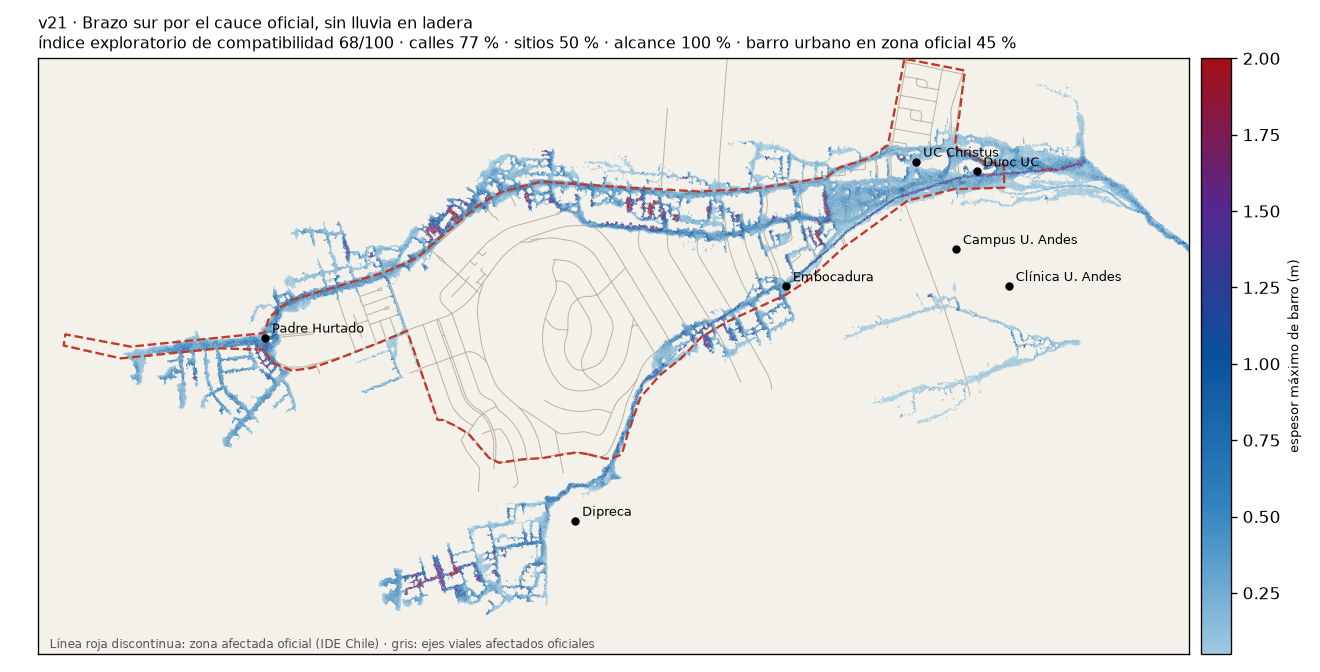
\includegraphics[width=\textwidth]{anexo/v21}\caption{Ficha v21: Brazo sur por el cauce oficial, sin lluvia en ladera.}\end{figure}

\paragraph{v19 · Brazo sur por el cauce oficial hasta Álvaro del Portillo + lluvia (paso fino).} \textbf{Qué prueba:} La hipótesis seleccionada (z02) con el brazo sur trazado según la cartografía oficial, para examinar si el flujo llega al campus y al Aula Magna. \textbf{Qué muestra:} Calculado: reproduce un desborde en la parte alta de Álvaro del Portillo y su descenso por la avenida, además de lo que logra z02. \textbf{Limitaciones del modelo:} El flujo simulado sigue por la avenida, de mayor pendiente ($\sim$8 \%) que el bosque hacia la Biblioteca ($\sim$4 \%), y no alcanza la depresión junto al edificio ni el punto de control del campus (1 cm). \textbf{Qué levanta:} En las microsimulaciones posteriores, el desborde supuesto no llega al patio con ninguno de los fluidos ensayados; el escenario más compatible supone escorrentía turbia de la ladera que, en el modelo, sigue La Plaza Sur y entra por un claro, con rasgos tallados que el relieve de 30 m no resuelve. \textbf{Estado:} IEC 71/100. Superada como ajuste por el escenario con aporte supuesto de escorrentía local (ver v32); no se determina el origen real del agua.

\begin{figure}[H]\centering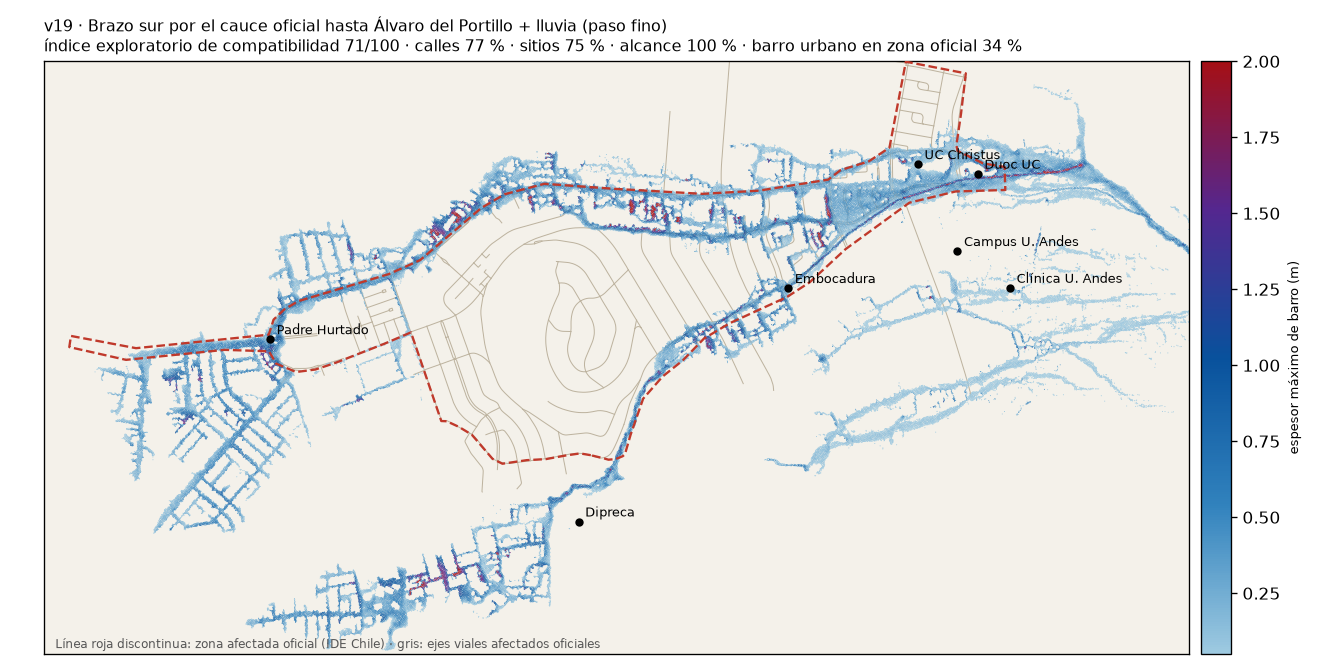
\includegraphics[width=\textwidth]{anexo/v19}\caption{Ficha v19: Brazo sur por el cauce oficial hasta Álvaro del Portillo + lluvia (paso fino).}\end{figure}

\subsection*{Colector de Bulnes Correa (escenarios hipotéticos)}

\paragraph{v17 · Escenario hipotético: capacidad supuesta del colector fijada en 30 m$^3$/s.} \textbf{Qué prueba:} Escenario hipotético con capacidad supuesta del colector fijada en 30 m$^3$/s y captura de toda la sección del cauce. No se dispuso de información pública sobre la capacidad y el estado reales del colector. \textbf{Qué muestra:} Calculado: el colector modelado alcanza la capacidad impuesta (retira 67,6 mil m$^3$ a 30 m$^3$/s) y Quebrada Honda se moja en el 62 \% de sus puntos. \textbf{Limitaciones del modelo:} — \textbf{Qué levanta:} En el modelo, con capacidad supuesta de 30 m$^3$/s, queda flujo superficial hacia Quebrada Honda. No es una evaluación de la obra real. \textbf{Estado:} Referencia inferior del intervalo explorado en estos escenarios: IEC 69/100.

\begin{figure}[H]\centering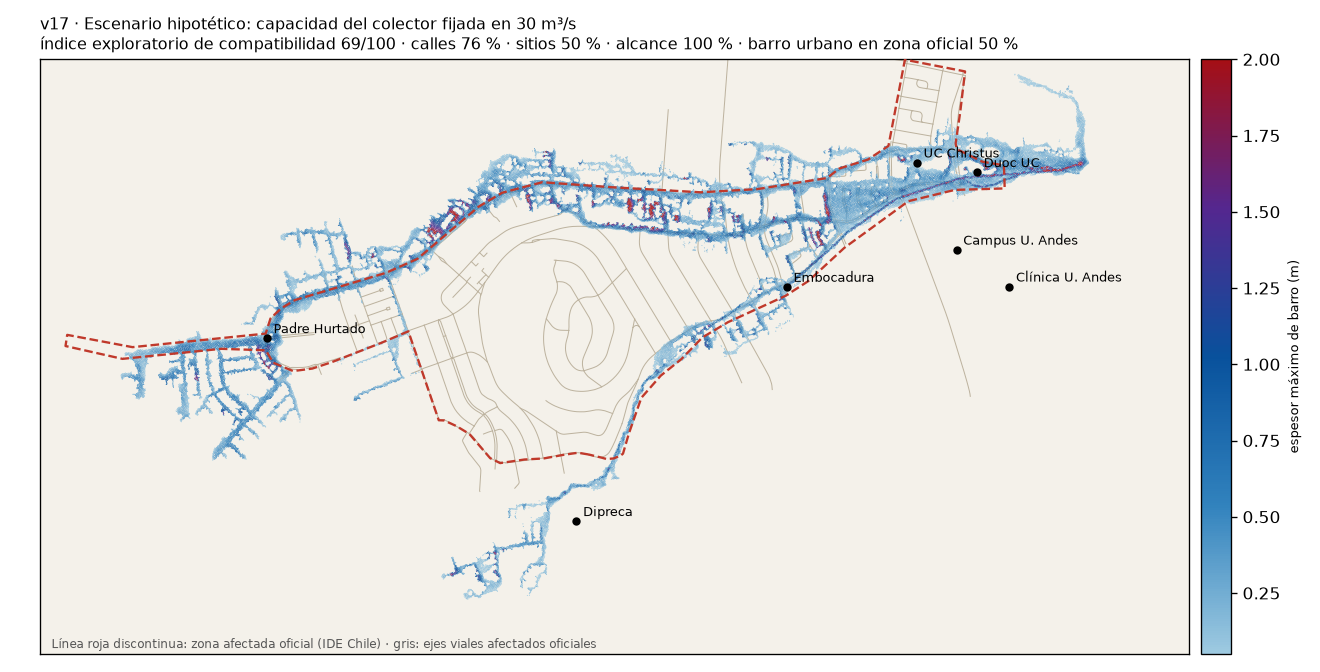
\includegraphics[width=\textwidth]{anexo/v17}\caption{Ficha v17: Escenario hipotético: capacidad supuesta del colector fijada en 30 m$^3$/s.}\end{figure}

\paragraph{v10 · Escenario hipotético: capacidad supuesta del colector fijada en 100 m$^3$/s.} \textbf{Qué prueba:} Escenario hipotético de gran capacidad con captura de toda la sección del cauce. \textbf{Qué muestra:} Calculado: el colector modelado retira unos 93 mil m$^3$ con un pico de $\sim$64 m$^3$/s y Quebrada Honda queda seca. Con 200 m$^3$/s el resultado es el mismo, porque el caudal calculado de llegada no supera $\sim$65 m$^3$/s. \textbf{Limitaciones del modelo:} El escenario no reproduce la inundación informada en Quebrada Honda; esta discrepancia no permite establecer cómo funcionó el colector real. \textbf{Qué levanta:} Bajo los supuestos ensayados y con captura completa, el análisis sitúa cerca de 65 m$^3$/s el umbral calculado de capacidad supuesta para retirar todo el flujo superficial en el modelo. Un radio de captura de 12 m dejaba pasar el flujo por el costado del sumidero: era un artefacto de representación, ya corregido. \textbf{Estado:} Referencia superior del intervalo explorado en estos escenarios: IEC 68/100.

\begin{figure}[H]\centering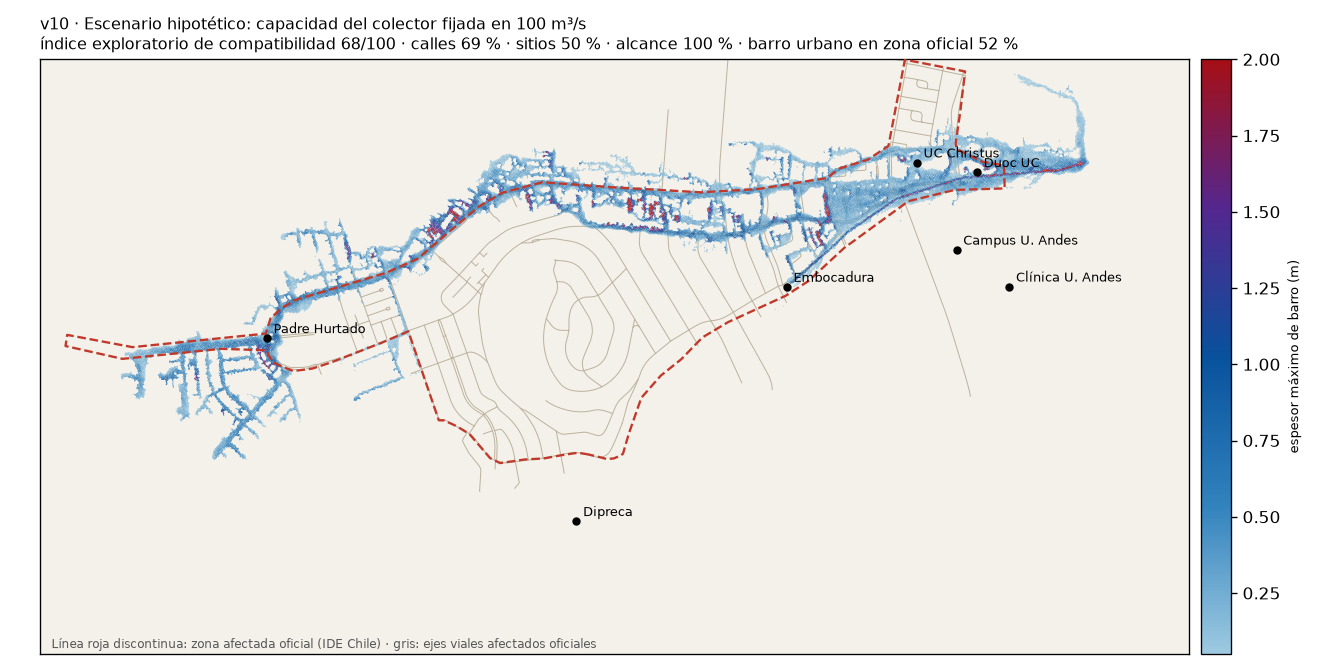
\includegraphics[width=\textwidth]{anexo/v10}\caption{Ficha v10: Escenario hipotético: capacidad supuesta del colector fijada en 100 m$^3$/s.}\end{figure}

\subsection*{Tipo de barro}

\paragraph{v08 · Barro espeso (Glenwood 1, Cv 0,45).} \textbf{Qué prueba:} Un barro más concentrado y viscoso (1.742 kg/m$^3$, fluencia 29 Pa). \textbf{Qué muestra:} Calculado: el frente se detiene a 396 m de Padre Hurtado. \textbf{Limitaciones del modelo:} No cumple el criterio de alcance. \textbf{Qué levanta:} Un material intermedio (Cv 0,43, v25) no reduce el barro fuera de la zona oficial; en todo el rango de Cv entre 0,24 y 0,48 (cuadratura de la concentración) el índice queda entre 71 y 73. \textbf{Estado:} Variante de mayor espesor: IEC 67/100.

\begin{figure}[H]\centering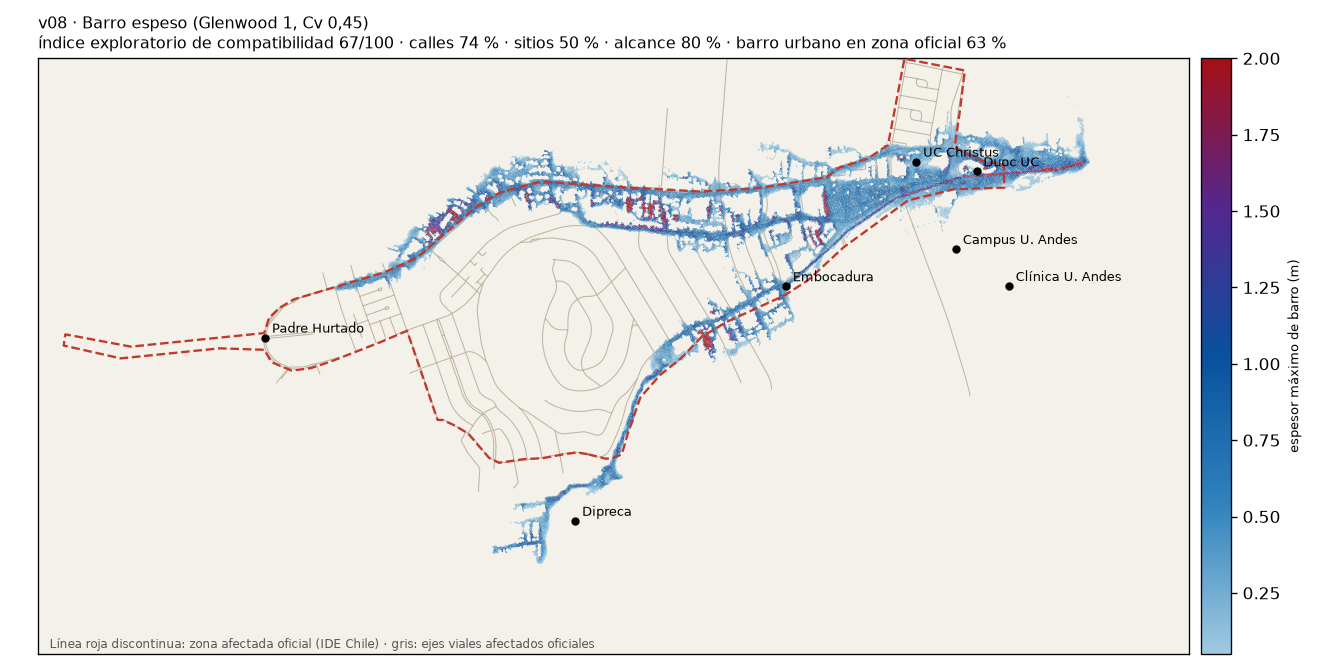
\includegraphics[width=\textwidth]{anexo/v08}\caption{Ficha v08: Barro espeso (Glenwood 1, Cv 0,45).}\end{figure}

\paragraph{v09 · Barro muy fluido (Aspen 2).} \textbf{Qué prueba:} Un barro más fluido que el de referencia. \textbf{Qué muestra:} Calculado: resultado parecido al de referencia (IEC 70/100), con algo más de barro dentro de la zona oficial. \textbf{Limitaciones del modelo:} No llega al sector sur (sin brazos sur ni lluvia). \textbf{Qué levanta:} El IEC varía poco entre los materiales ensayados; esa variación no resume por sí sola los cambios de alcance, profundidad o velocidad. \textbf{Estado:} Sensibilidad del índice al material: baja. IEC 70/100.

\begin{figure}[H]\centering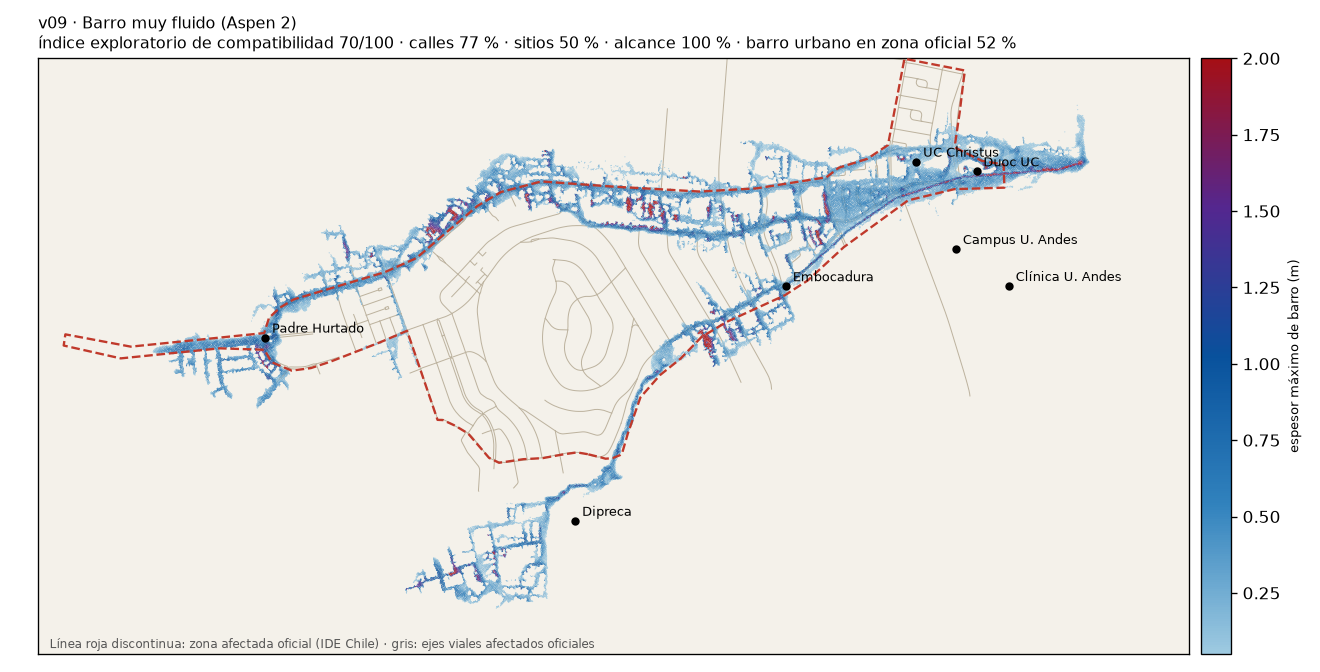
\includegraphics[width=\textwidth]{anexo/v09}\caption{Ficha v09: Barro muy fluido (Aspen 2).}\end{figure}

\subsection*{Terreno anterior (primera generación)}

\paragraph{e04 · Cauce + colector con capacidad nula supuesta, terreno con 1.103 edificios.} \textbf{Qué prueba:} La configuración seleccionada en la primera generación (9 de octubre), con solo 1.103 edificios representados y el criterio de perímetro de prensa. \textbf{Qué muestra:} Calculado: el flujo se reparte más en superficie (93 ha dentro de la zona oficial) con láminas más delgadas y llega a Padre Hurtado. \textbf{Limitaciones del modelo:} Calcula solo 0,3 m en el entorno de la UC Christus (Cadena 3 informó cerca de 1 m en urgencias). \textbf{Qué levanta:} Representar todos los edificios cambió los resultados; la representación mediante bloques impermeables podría intensificar el encauzamiento respecto de una que permita retención en edificios (v26). \textbf{Estado:} Superada por las simulaciones con la ciudad completa: IEC 68/100.

\begin{figure}[H]\centering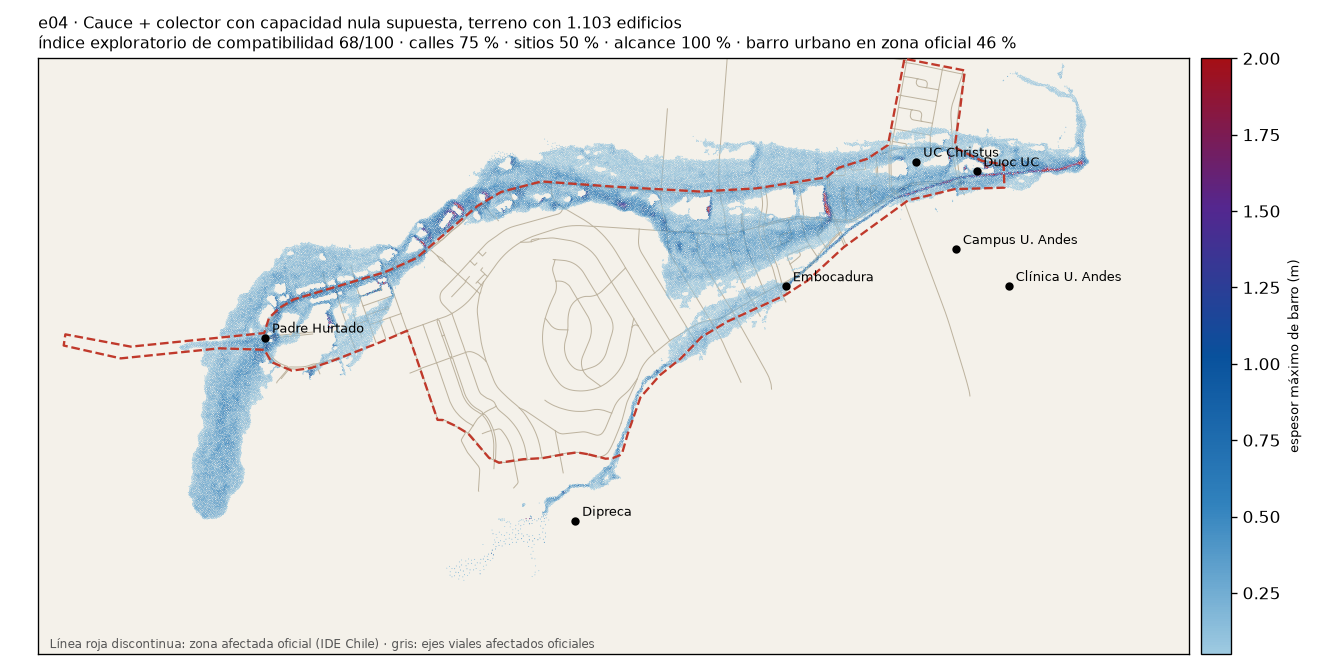
\includegraphics[width=\textwidth]{anexo/e04}\caption{Ficha e04: Cauce + colector con capacidad nula supuesta, terreno con 1.103 edificios.}\end{figure}

\paragraph{f03 · Abanico + embocadura + lluvia en ladera, terreno anterior.} \textbf{Qué prueba:} La primera simulación con lluvia sobre la ladera, con el terreno anterior. \textbf{Qué muestra:} Calculado: fue la primera en producir flujo junto a la Clínica U. de los Andes y en La Plaza Sur. \textbf{Limitaciones del modelo:} Espesor bajo en el entorno de la UC Christus y extensión fuera de la zona oficial. \textbf{Qué levanta:} Dio origen a la hipótesis seleccionada para la prueba reservada (cauce + brazos sur + lluvia, z02). \textbf{Estado:} IEC 71/100.

\begin{figure}[H]\centering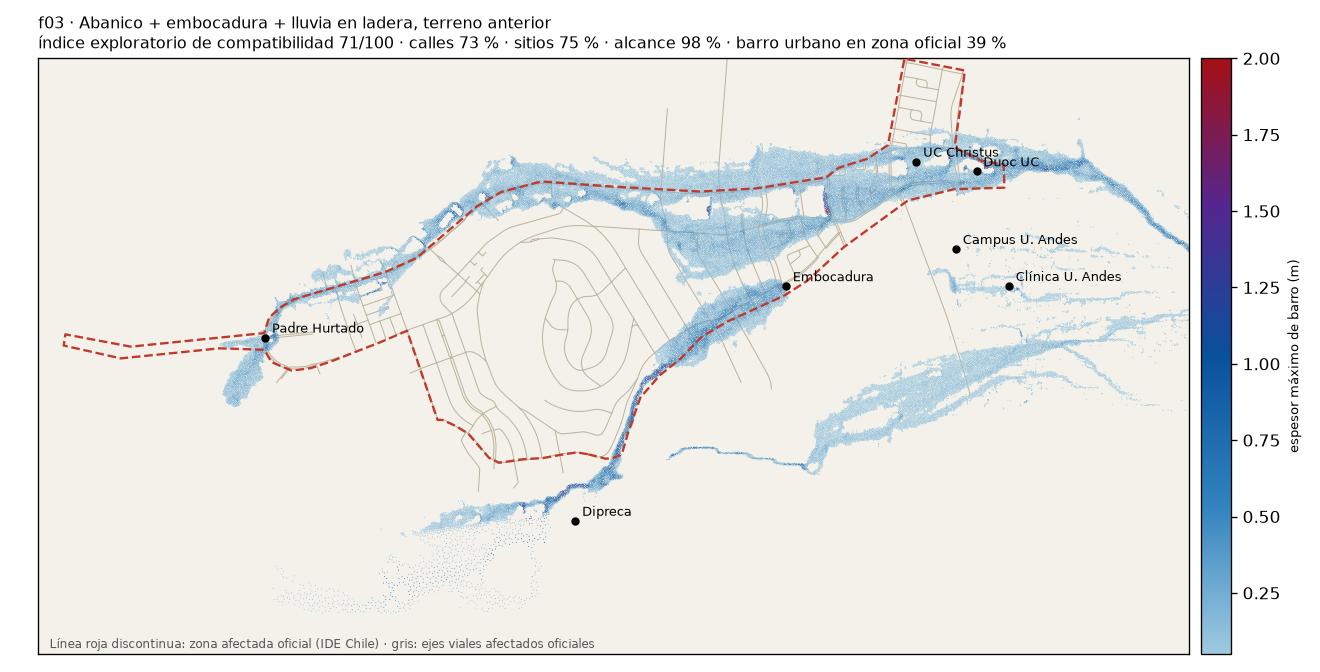
\includegraphics[width=\textwidth]{anexo/f03}\caption{Ficha f03: Abanico + embocadura + lluvia en ladera, terreno anterior.}\end{figure}

\paragraph{e03 · Solo desborde en la embocadura (H2).} \textbf{Qué prueba:} Una entrada superficial de todo el volumen supuesto en Francisco Bulnes Correa, sin inferir el funcionamiento real del canal. \textbf{Qué muestra:} Calculado: moja Quebrada Honda, pero nada del abanico. \textbf{Limitaciones del modelo:} No reproduce General Blanche, Camino El Alba, Duoc UC ni la UC Christus. \textbf{Qué levanta:} El Desconcierto recoge un desborde en Bulnes Correa informado por Carabineros. La simulación e03 no reproduce por sí sola el conjunto de observaciones. \textbf{Estado:} No reproduce por sí sola el conjunto de observaciones bajo los supuestos y el terreno de e03: IEC 16/100.

\begin{figure}[H]\centering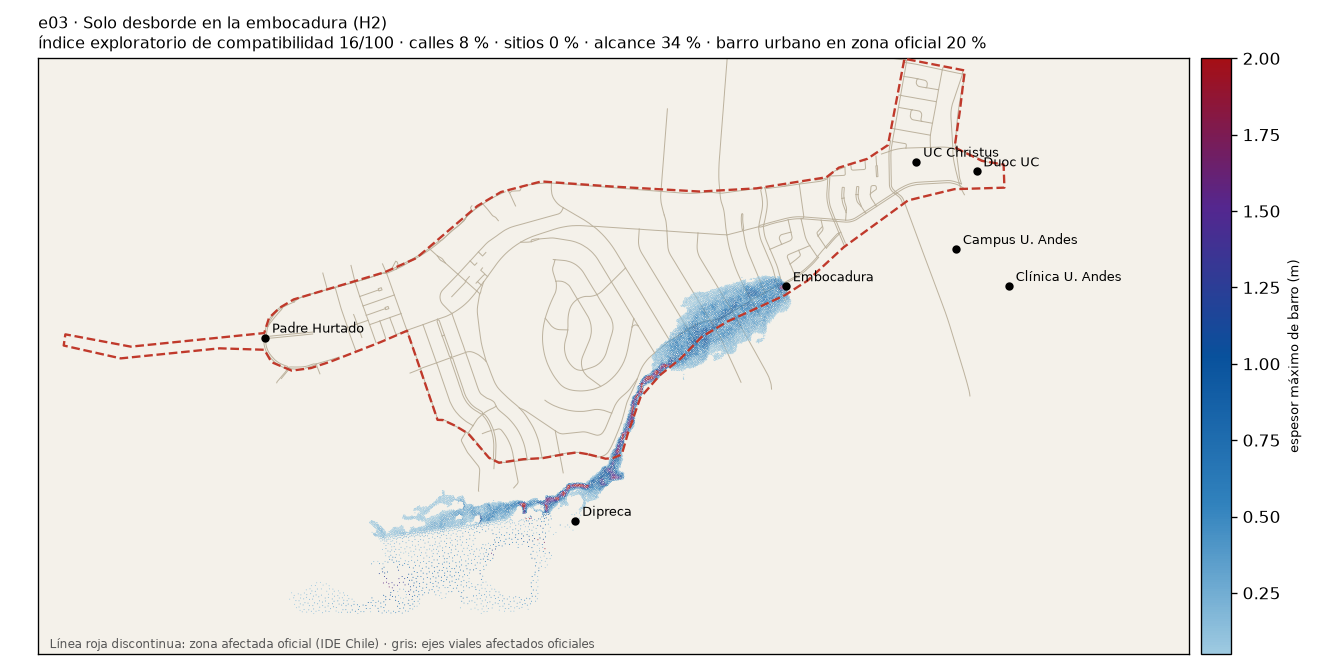
\includegraphics[width=\textwidth]{anexo/e03}\caption{Ficha e03: Solo desborde en la embocadura (H2).}\end{figure}
